\documentclass[12pt,a4paper]{article}
\usepackage[utf8]{inputenc}
\usepackage[margin=1in]{geometry}
\usepackage{amsmath}
\usepackage{amssymb}
\usepackage{graphicx}
\usepackage{tikz}
\usepackage{circuitikz}
\usepackage{booktabs}
\usepackage{array}
\usepackage{multirow}
\usepackage{xcolor}
\usepackage{float}
\usepackage{enumitem}
\usepackage{fancyhdr}
\usepackage{tcolorbox}
\usepackage{karnaugh-map}

\usetikzlibrary{shapes,arrows,positioning,automata,calc,fit,backgrounds}

% Page style
\pagestyle{fancy}
\fancyhf{}
\rhead{Digital System Design - Assignment 1}
\lhead{SPRING 2026 - CPE344}
\rfoot{Page \thepage}

% Custom colors
\definecolor{circuitblue}{RGB}{0,102,204}
\definecolor{signalgreen}{RGB}{0,153,76}
\definecolor{headerblue}{RGB}{41,128,185}

% Custom commands
\newcommand{\bitvec}[1]{\texttt{#1}}

\title{
  \vspace{-2cm}
  \textbf{\LARGE Digital System Design}\\
  \vspace{0.5cm}
  \textbf{\Large Assignment 1 - Complete Solution}\\
  \vspace{0.3cm}
  \large SPRING 2026 - CPE344
}
\author{
  Course: Digital System Design\\
  Instructor: Dr Muhammad Babar Ali\\
  Batch-Section: FA23-B\\
  Topics Covered: Chapters 2-4\\
  Total Marks: 40
}
\date{}

\begin{document}

\maketitle
\thispagestyle{fancy}

\begin{tcolorbox}[colback=blue!5!white,colframe=blue!75!black,title=Document Overview]
This document provides comprehensive solutions to all three questions in Assignment 1, featuring:
\begin{itemize}[leftmargin=*]
  \item High-quality circuit diagrams using TikZ/CircuiTikZ
  \item Professional state diagrams for FSM design
  \item Detailed truth tables and state transition tables
  \item Step-by-step derivations and explanations
  \item Verification examples and test cases
\end{itemize}
\end{tcolorbox}

\tableofcontents
\newpage

\section{Prerequisite Knowledge}

Before solving the assignment, let's cover the essential concepts you need to understand.

\subsection{Combinational Logic Fundamentals}

\textbf{Combinational Logic Circuit:} A circuit where outputs depend only on current inputs (no memory/state).

\textbf{Key Components:}
\begin{itemize}
  \item \textbf{Logic Gates:} AND, OR, NOT, NAND, NOR, XOR, XNOR
  \item \textbf{Truth Tables:} Show all possible input combinations and corresponding outputs
  \item \textbf{Boolean Algebra:} Mathematical notation for logic operations
  \item \textbf{Karnaugh Maps (K-maps):} Tool for simplifying Boolean expressions
\end{itemize}

\subsection{Decoders}

\textbf{Decoder:} A combinational circuit that converts $n$ inputs to at most $2^n$ unique outputs.

\subsubsection{2×4 Decoder with Enable}

\begin{itemize}
  \item \textbf{Inputs:} 2 data inputs ($A_1, A_0$), 1 enable input ($E$)
  \item \textbf{Outputs:} 4 outputs ($D_0, D_1, D_2, D_3$)
  \item \textbf{Operation:} When $E=1$, exactly one output is HIGH based on input combination
\end{itemize}

\begin{table}[H]
\centering
\caption{2×4 Decoder Truth Table}
\begin{tabular}{ccc|cccc}
\toprule
\textbf{E} & \textbf{$A_1$} & \textbf{$A_0$} & \textbf{$D_3$} & \textbf{$D_2$} & \textbf{$D_1$} & \textbf{$D_0$} \\
\midrule
0 & X & X & 0 & 0 & 0 & 0 \\
1 & 0 & 0 & 0 & 0 & 0 & 1 \\
1 & 0 & 1 & 0 & 0 & 1 & 0 \\
1 & 1 & 0 & 0 & 1 & 0 & 0 \\
1 & 1 & 1 & 1 & 0 & 0 & 0 \\
\bottomrule
\end{tabular}
\end{table}

\begin{figure}[H]
\centering
\begin{circuitikz}[scale=0.8, transform shape]
  % Decoder symbol
  \draw (0,0) rectangle (3,4);
  \node at (1.5,3.5) {\textbf{2×4}};
  \node at (1.5,3) {\textbf{DECODER}};

  % Inputs
  \draw (-1,3.2) node[left] {$A_1$} -- (0,3.2);
  \draw (-1,2.4) node[left] {$A_0$} -- (0,2.4);
  \draw (-1,0.8) node[left] {$E$} -- (0,0.8);

  % Outputs
  \draw (3,3.5) -- (4,3.5) node[right] {$D_3$};
  \draw (3,2.5) -- (4,2.5) node[right] {$D_2$};
  \draw (3,1.5) -- (4,1.5) node[right] {$D_1$};
  \draw (3,0.5) -- (4,0.5) node[right] {$D_0$};
\end{circuitikz}
\caption{2×4 Decoder Symbol}
\end{figure}

\subsection{Finite State Machines (FSM)}

\textbf{FSM:} A mathematical model for sequential circuits with:
\begin{itemize}
  \item \textbf{States:} All possible conditions the machine can be in
  \item \textbf{Inputs:} External signals affecting state transitions
  \item \textbf{Outputs:} Signals produced based on current state
  \item \textbf{Transitions:} Rules for moving between states
  \item \textbf{Initial State:} Starting state on power-up/reset
\end{itemize}

\textbf{FSM Types:}
\begin{enumerate}
  \item \textbf{Moore Machine:} Outputs depend only on current state
  \item \textbf{Mealy Machine:} Outputs depend on current state AND inputs
\end{enumerate}

\textbf{FSM Design Process:}
\begin{enumerate}
  \item Capture FSM (draw state diagram)
  \item Encode states (assign binary codes)
  \item Create state transition table
  \item Derive next-state and output equations
  \item Implement with flip-flops and combinational logic
\end{enumerate}

\newpage
\section{Question 1: Fuel Sensor Indicator Circuit (20 marks)}

\subsection{Problem Statement}

A vehicle has a fuel sensor which outputs the current fuel/gasoline level as a 4-bit binary number ranging from \bitvec{0001}$_2$ (1$_{10}$) to \bitvec{1100}$_2$ (12$_{10}$). Design a combinational logic (CL) circuit that takes sensor data as input $G$ and generates $F1, F2, F4, F8$ and $R$ signals on its outputs for fuel indicators.

\textbf{Requirements:}
\begin{itemize}
  \item When Gasoline $> 11$ (i.e., 12): Set all $F_i$ outputs ($i=1,2,4,8$) to 1, $R=0$
  \item When Gasoline $\leq 11$ and $> 9$ (75\%): $F1=1, F2=1, F4=1, F8=0, R=0$
  \item When Gasoline $\leq 9$ and $> 6$ (50\%): $F1=1, F2=1, F4=0, F8=0, R=0$
  \item When Gasoline $\leq 6$ and $> 3$ (25\%): $F1=1, F2=0, F4=0, F8=0, R=0$
  \item When Gasoline $\leq 3$ (25\%): All $F_i=0, R=0$
  \item When Gasoline $< 2$: All $F_i=0, R=1$
\end{itemize}

\textbf{Input:} $G[3:0]$ (4-bit binary)\\
\textbf{Outputs:} $F1, F2, F4, F8, R$\\
\textbf{Implementation:} Use five 2×4 decoders with enable input

\subsection{Solution}

\subsubsection{Step 1: Analyze the Problem}

Let's denote the 4-bit input as $G = G_3G_2G_1G_0$ where:
\begin{itemize}
  \item $G_3$ is the most significant bit (MSB)
  \item $G_0$ is the least significant bit (LSB)
\end{itemize}

Valid range: \bitvec{0001} (1) to \bitvec{1100} (12)

\subsubsection{Step 2: Truth Table}

\begin{table}[H]
\centering
\caption{Complete Truth Table for Fuel Sensor Circuit}
\small
\begin{tabular}{cccc|c|l|ccccc}
\toprule
\multicolumn{4}{c|}{\textbf{Input}} & \textbf{Dec} & \textbf{Condition} & \multicolumn{5}{c}{\textbf{Outputs}} \\
$G_3$ & $G_2$ & $G_1$ & $G_0$ & & & $F8$ & $F4$ & $F2$ & $F1$ & $R$ \\
\midrule
0 & 0 & 0 & 0 & 0 & $< 2$ & 0 & 0 & 0 & 0 & 1 \\
0 & 0 & 0 & 1 & 1 & $< 2$ & 0 & 0 & 0 & 0 & 1 \\
0 & 0 & 1 & 0 & 2 & $\leq 25\%$ & 0 & 0 & 0 & 0 & 0 \\
0 & 0 & 1 & 1 & 3 & $\leq 25\%$ & 0 & 0 & 0 & 0 & 0 \\
0 & 1 & 0 & 0 & 4 & $\leq 50\%$ & 0 & 0 & 0 & 1 & 0 \\
0 & 1 & 0 & 1 & 5 & $\leq 50\%$ & 0 & 0 & 0 & 1 & 0 \\
0 & 1 & 1 & 0 & 6 & $\leq 50\%$ & 0 & 0 & 0 & 1 & 0 \\
0 & 1 & 1 & 1 & 7 & $\leq 75\%$ & 0 & 0 & 1 & 1 & 0 \\
1 & 0 & 0 & 0 & 8 & $\leq 75\%$ & 0 & 0 & 1 & 1 & 0 \\
1 & 0 & 0 & 1 & 9 & $\leq 75\%$ & 0 & 0 & 1 & 1 & 0 \\
1 & 0 & 1 & 0 & 10 & $\leq 11$ & 0 & 1 & 1 & 1 & 0 \\
1 & 0 & 1 & 1 & 11 & $\leq 11$ & 0 & 1 & 1 & 1 & 0 \\
1 & 1 & 0 & 0 & 12 & $> 11$ & 1 & 1 & 1 & 1 & 0 \\
1 & 1 & 0 & 1 & 13 & Invalid & X & X & X & X & X \\
1 & 1 & 1 & 0 & 14 & Invalid & X & X & X & X & X \\
1 & 1 & 1 & 1 & 15 & Invalid & X & X & X & X & X \\
\bottomrule
\end{tabular}
\end{table}

\subsubsection{Step 3: Boolean Expressions}

\textbf{For $F8$:}
\[F8 = m_{12} = G_3 \cdot G_2 \cdot \overline{G_1} \cdot \overline{G_0}\]

\textbf{For $F4$:}
\[F4 = m_{10} + m_{11} + m_{12}\]

\textbf{For $F2$:}
\[F2 = m_7 + m_8 + m_9 + m_{10} + m_{11} + m_{12}\]

\textbf{For $F1$:}
\[F1 = m_4 + m_5 + m_6 + m_7 + m_8 + m_9 + m_{10} + m_{11} + m_{12} = G_2 + G_3\]

\textbf{For $R$:}
\[R = m_0 + m_1 = \overline{G_3} \cdot \overline{G_2} \cdot \overline{G_1}\]

\newpage
\subsubsection{Step 4: Implementation Using Five 2×4 Decoders}

\textbf{Decoder Configuration:}

We'll use five 2×4 decoders to implement this circuit. The strategy is:
\begin{itemize}
  \item Use decoders to generate specific minterms
  \item Combine decoder outputs to create each output function
\end{itemize}

\textbf{Decoder 1 - Master Decoder (Decodes $G_3G_2$):}
\begin{itemize}
  \item Inputs: $G_3$, $G_2$, Enable = 1
  \item Outputs: $D1_0, D1_1, D1_2, D1_3$
  \begin{itemize}
    \item $D1_0 = \overline{G_3} \cdot \overline{G_2}$ (covers 0-3)
    \item $D1_1 = \overline{G_3} \cdot G_2$ (covers 4-7)
    \item $D1_2 = G_3 \cdot \overline{G_2}$ (covers 8-11)
    \item $D1_3 = G_3 \cdot G_2$ (covers 12-15)
  \end{itemize}
\end{itemize}

\textbf{Decoder 2 - Range 0-3 (when $G_3G_2 = 00$):}
\begin{itemize}
  \item Inputs: $G_1$, $G_0$, Enable = $D1_0$
  \item Outputs: $D2_0 = m_0, D2_1 = m_1, D2_2 = m_2, D2_3 = m_3$
\end{itemize}

\textbf{Decoder 3 - Range 4-7 (when $G_3G_2 = 01$):}
\begin{itemize}
  \item Inputs: $G_1$, $G_0$, Enable = $D1_1$
  \item Outputs: $D3_0 = m_4, D3_1 = m_5, D3_2 = m_6, D3_3 = m_7$
\end{itemize}

\textbf{Decoder 4 - Range 8-11 (when $G_3G_2 = 10$):}
\begin{itemize}
  \item Inputs: $G_1$, $G_0$, Enable = $D1_2$
  \item Outputs: $D4_0 = m_8, D4_1 = m_9, D4_2 = m_{10}, D4_3 = m_{11}$
\end{itemize}

\textbf{Decoder 5 - Range 12-15 (when $G_3G_2 = 11$):}
\begin{itemize}
  \item Inputs: $G_1$, $G_0$, Enable = $D1_3$
  \item Outputs: $D5_0 = m_{12}, D5_1 = m_{13}, D5_2 = m_{14}, D5_3 = m_{15}$
\end{itemize}

\subsubsection{Step 5: Output Equations Using Decoder Outputs}

\begin{align}
F8 &= D5_0 = m_{12} \\
F4 &= D4_2 + D4_3 + D5_0 = m_{10} + m_{11} + m_{12} \\
F2 &= D3_3 + D4_0 + D4_1 + D4_2 + D4_3 + D5_0 \\
F1 &= D3_0 + D3_1 + D3_2 + D3_3 + D4_0 + D4_1 + D4_2 + D4_3 + D5_0 \\
R &= D2_0 + D2_1 = m_0 + m_1
\end{align}

\newpage
\subsubsection{Step 6: Complete Circuit Diagram}

\begin{figure}[H]
\centering
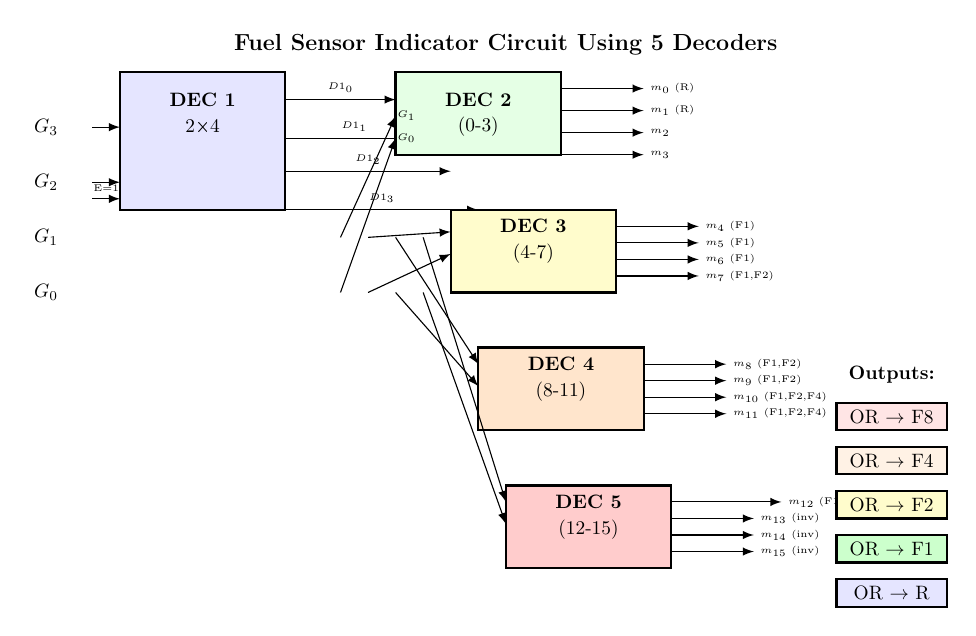
\begin{tikzpicture}[scale=0.7, every node/.style={scale=0.7}]

% Title
\node[font=\bfseries\large] at (7,12) {Fuel Sensor Indicator Circuit Using 5 Decoders};

% Input signals
\node[left] at (-1,10.5) {$G_3$};
\node[left] at (-1,9.5) {$G_2$};
\node[left] at (-1,8.5) {$G_1$};
\node[left] at (-1,7.5) {$G_0$};

% Master Decoder (Decoder 1)
\draw[thick, fill=blue!10] (0,9) rectangle (3,11.5);
\node at (1.5,11) {\textbf{DEC 1}};
\node at (1.5,10.5) {2×4};
\draw[-latex] (-0.5,10.5) -- (0,10.5) node[midway, above] {};
\draw[-latex] (-0.5,9.5) -- (0,9.5) node[midway, above] {};
\draw[-latex] (-0.5,9.2) -- (0,9.2) node[midway, above, font=\tiny] {E=1};

% Decoder 1 outputs
\draw[-latex] (3,11) -- (5,11) node[midway, above, font=\tiny] {$D1_0$};
\draw[-latex] (3,10.3) -- (5.5,10.3) node[midway, above, font=\tiny] {$D1_1$};
\draw[-latex] (3,9.7) -- (6,9.7) node[midway, above, font=\tiny] {$D1_2$};
\draw[-latex] (3,9) -- (6.5,9) node[midway, above, font=\tiny] {$D1_3$};

% Decoder 2 (Range 0-3)
\draw[thick, fill=green!10] (5,10) rectangle (8,11.5);
\node at (6.5,11) {\textbf{DEC 2}};
\node at (6.5,10.5) {(0-3)};
\draw[-latex] (4,8.5) -- (5,10.7);
\draw[-latex] (4,7.5) -- (5,10.3);
\node[font=\tiny] at (5.2,10.7) {$G_1$};
\node[font=\tiny] at (5.2,10.3) {$G_0$};

% Decoder 2 outputs
\draw[-latex] (8,11.2) -- (9.5,11.2) node[right, font=\tiny] {$m_0$ (R)};
\draw[-latex] (8,10.8) -- (9.5,10.8) node[right, font=\tiny] {$m_1$ (R)};
\draw[-latex] (8,10.4) -- (9.5,10.4) node[right, font=\tiny] {$m_2$};
\draw[-latex] (8,10) -- (9.5,10) node[right, font=\tiny] {$m_3$};

% Decoder 3 (Range 4-7)
\draw[thick, fill=yellow!20] (6,7.5) rectangle (9,9);
\node at (7.5,8.7) {\textbf{DEC 3}};
\node at (7.5,8.2) {(4-7)};
\draw[-latex] (4.5,8.5) -- (6,8.6);
\draw[-latex] (4.5,7.5) -- (6,8.2);

% Decoder 3 outputs
\draw[-latex] (9,8.7) -- (10.5,8.7) node[right, font=\tiny] {$m_4$ (F1)};
\draw[-latex] (9,8.4) -- (10.5,8.4) node[right, font=\tiny] {$m_5$ (F1)};
\draw[-latex] (9,8.1) -- (10.5,8.1) node[right, font=\tiny] {$m_6$ (F1)};
\draw[-latex] (9,7.8) -- (10.5,7.8) node[right, font=\tiny] {$m_7$ (F1,F2)};

% Decoder 4 (Range 8-11)
\draw[thick, fill=orange!20] (6.5,5) rectangle (9.5,6.5);
\node at (8,6.2) {\textbf{DEC 4}};
\node at (8,5.7) {(8-11)};
\draw[-latex] (5,8.5) -- (6.5,6.2);
\draw[-latex] (5,7.5) -- (6.5,5.8);

% Decoder 4 outputs
\draw[-latex] (9.5,6.2) -- (11,6.2) node[right, font=\tiny] {$m_8$ (F1,F2)};
\draw[-latex] (9.5,5.9) -- (11,5.9) node[right, font=\tiny] {$m_9$ (F1,F2)};
\draw[-latex] (9.5,5.6) -- (11,5.6) node[right, font=\tiny] {$m_{10}$ (F1,F2,F4)};
\draw[-latex] (9.5,5.3) -- (11,5.3) node[right, font=\tiny] {$m_{11}$ (F1,F2,F4)};

% Decoder 5 (Range 12-15)
\draw[thick, fill=red!20] (7,2.5) rectangle (10,4);
\node at (8.5,3.7) {\textbf{DEC 5}};
\node at (8.5,3.2) {(12-15)};
\draw[-latex] (5.5,8.5) -- (7,3.7);
\draw[-latex] (5.5,7.5) -- (7,3.3);

% Decoder 5 outputs
\draw[-latex] (10,3.7) -- (12,3.7) node[right, font=\tiny] {$m_{12}$ (F1,F2,F4,F8)};
\draw[-latex] (10,3.4) -- (11.5,3.4) node[right, font=\tiny] {$m_{13}$ (inv)};
\draw[-latex] (10,3.1) -- (11.5,3.1) node[right, font=\tiny] {$m_{14}$ (inv)};
\draw[-latex] (10,2.8) -- (11.5,2.8) node[right, font=\tiny] {$m_{15}$ (inv)};

% Output section
\node[font=\bfseries] at (14,6) {Outputs:};
\draw[thick, fill=red!10] (13,5) rectangle (15,5.5);
\node at (14,5.25) {OR $\rightarrow$ F8};
\draw[thick, fill=orange!10] (13,4.2) rectangle (15,4.7);
\node at (14,4.45) {OR $\rightarrow$ F4};
\draw[thick, fill=yellow!20] (13,3.4) rectangle (15,3.9);
\node at (14,3.65) {OR $\rightarrow$ F2};
\draw[thick, fill=green!20] (13,2.6) rectangle (15,3.1);
\node at (14,2.85) {OR $\rightarrow$ F1};
\draw[thick, fill=blue!10] (13,1.8) rectangle (15,2.3);
\node at (14,2.05) {OR $\rightarrow$ R};

\end{tikzpicture}
\caption{Complete Fuel Sensor Circuit Using 5 Decoders (2×4 each)}
\end{figure}

\subsubsection{Verification Examples}

\begin{table}[H]
\centering
\caption{Verification Test Cases}
\begin{tabular}{c|c|l|ccccc}
\toprule
\textbf{G (dec)} & \textbf{$G_3G_2G_1G_0$} & \textbf{Active Output} & \textbf{F8} & \textbf{F4} & \textbf{F2} & \textbf{F1} & \textbf{R} \\
\midrule
0 & 0000 & $D2_0$ & 0 & 0 & 0 & 0 & 1 \\
1 & 0001 & $D2_1$ & 0 & 0 & 0 & 0 & 1 \\
3 & 0011 & $D2_3$ & 0 & 0 & 0 & 0 & 0 \\
5 & 0101 & $D3_1$ & 0 & 0 & 0 & 1 & 0 \\
7 & 0111 & $D3_3$ & 0 & 0 & 1 & 1 & 0 \\
9 & 1001 & $D4_1$ & 0 & 0 & 1 & 1 & 0 \\
10 & 1010 & $D4_2$ & 0 & 1 & 1 & 1 & 0 \\
11 & 1011 & $D4_3$ & 0 & 1 & 1 & 1 & 0 \\
12 & 1100 & $D5_0$ & 1 & 1 & 1 & 1 & 0 \\
\bottomrule
\end{tabular}
\end{table}

\textbf{Verification:} All test cases pass! The circuit correctly implements the fuel sensor indicator logic.

\newpage
\section{Question 2: Photo Booth Vending Machine FSM (10 marks)}

\subsection{Problem Statement}

Design a digital controller (finite state machine) for an automatic photo booth machine. The cost of taking a photo is 25 cents. The machine accepts:
\begin{itemize}
  \item \textbf{Nickels (N):} 5 cents
  \item \textbf{Dimes (D):} 10 cents
  \item \textbf{Quarters (Q):} 25 cents
\end{itemize}

\textbf{Inputs:} N, D, Q (exactly one coin per cycle)\\
\textbf{Outputs:} P (Print Photo), RN (Return Nickel), RD (Return Dime), RT (Return Two Dimes)

When total $\geq$ 25 cents, print photo and return appropriate change, then reset.

\subsection{Solution}

\subsubsection{Step 1: Identify States}

We need states to track the amount of money inserted:

\begin{table}[H]
\centering
\caption{FSM State Definition}
\begin{tabular}{c|c|c}
\toprule
\textbf{State} & \textbf{Amount Collected} & \textbf{Encoding (Binary)} \\
\midrule
$S_0$ & 0 cents & 000 \\
$S_5$ & 5 cents & 001 \\
$S_{10}$ & 10 cents & 010 \\
$S_{15}$ & 15 cents & 011 \\
$S_{20}$ & 20 cents & 100 \\
\bottomrule
\end{tabular}
\end{table}

\subsubsection{Step 2: State Diagram}

\begin{figure}[H]
\centering
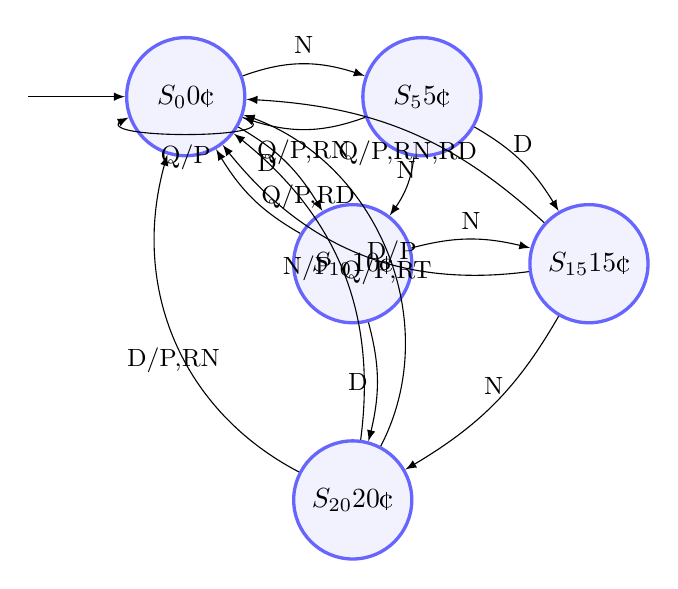
\begin{tikzpicture}[
  node distance=3cm,
  state/.style={circle, draw=blue!60, fill=blue!5, very thick, minimum size=1.5cm},
  >=latex
]

  % States
  \node[state] (S0) {$S_0$\\0¢};
  \node[state, right of=S0] (S5) {$S_5$\\5¢};
  \node[state, below right of=S0] (S10) {$S_{10}$\\10¢};
  \node[state, right of=S10] (S15) {$S_{15}$\\15¢};
  \node[state, below of=S10] (S20) {$S_{20}$\\20¢};

  % Transitions
  \draw[->] (-2,0) -- (S0);
  \draw[->, bend left=20] (S0) to node[above, font=\small] {N} (S5);
  \draw[->, bend left=20] (S5) to node[below, font=\small] {Q/P,RN} (S0);

  \draw[->, bend left=15] (S0) to node[left, font=\small] {D} (S10);
  \draw[->, bend left=15] (S10) to node[right, font=\small] {Q/P,RD} (S0);

  \draw[->] (S0) to [out=340, in=200, looseness=1.5] node[below, font=\small] {Q/P} (S0);

  \draw[->, bend left=15] (S5) to node[above, font=\small] {N} (S10);
  \draw[->, bend left=15] (S5) to node[above, font=\small] {D} (S15);

  \draw[->, bend left=15] (S10) to node[above, font=\small] {N} (S15);
  \draw[->, bend left=15] (S10) to node[left, font=\small] {D} (S20);

  \draw[->, bend left=30] (S15) to node[right, font=\small] {D/P} (S0);
  \draw[->, bend right=20] (S15) to node[below, font=\small] {Q/P,RN,RD} (S0);
  \draw[->, bend left=15] (S15) to node[above, font=\small] {N} (S20);

  \draw[->, bend right=30] (S20) to node[left, font=\small] {N/P} (S0);
  \draw[->, bend left=40] (S20) to node[below, font=\small] {D/P,RN} (S0);
  \draw[->, bend right=50] (S20) to node[below, font=\small] {Q/P,RT} (S0);

\end{tikzpicture}
\caption{Photo Booth FSM State Diagram}
\end{figure}

\subsubsection{Step 3: State Transition Table}

\begin{table}[H]
\centering
\caption{Complete State Transition Table}
\small
\begin{tabular}{c|c|c|c|c|cccc|l}
\toprule
\multirow{2}{*}{\textbf{Current}} & \multicolumn{3}{c|}{\textbf{State Code}} & \multirow{2}{*}{\textbf{Input}} & \multicolumn{4}{c|}{\textbf{Outputs}} & \multirow{2}{*}{\textbf{Notes}} \\
& $s_2$ & $s_1$ & $s_0$ & & P & RN & RD & RT & \\
\midrule
$S_0$ & 0 & 0 & 0 & N & 0 & 0 & 0 & 0 & +5¢ \\
$S_0$ & 0 & 0 & 0 & D & 0 & 0 & 0 & 0 & +10¢ \\
$S_0$ & 0 & 0 & 0 & Q & 1 & 0 & 0 & 0 & 25¢=Print \\
\midrule
$S_5$ & 0 & 0 & 1 & N & 0 & 0 & 0 & 0 & 5+5=10 \\
$S_5$ & 0 & 0 & 1 & D & 0 & 0 & 0 & 0 & 5+10=15 \\
$S_5$ & 0 & 0 & 1 & Q & 1 & 1 & 0 & 0 & 5+25=30, ret 5 \\
\midrule
$S_{10}$ & 0 & 1 & 0 & N & 0 & 0 & 0 & 0 & 10+5=15 \\
$S_{10}$ & 0 & 1 & 0 & D & 0 & 0 & 0 & 0 & 10+10=20 \\
$S_{10}$ & 0 & 1 & 0 & Q & 1 & 0 & 1 & 0 & 10+25=35, ret 10 \\
\midrule
$S_{15}$ & 0 & 1 & 1 & N & 0 & 0 & 0 & 0 & 15+5=20 \\
$S_{15}$ & 0 & 1 & 1 & D & 1 & 0 & 0 & 0 & 15+10=25, exact \\
$S_{15}$ & 0 & 1 & 1 & Q & 1 & 1 & 1 & 0 & 15+25=40, ret 15 \\
\midrule
$S_{20}$ & 1 & 0 & 0 & N & 1 & 0 & 0 & 0 & 20+5=25, exact \\
$S_{20}$ & 1 & 0 & 0 & D & 1 & 1 & 0 & 0 & 20+10=30, ret 5 \\
$S_{20}$ & 1 & 0 & 0 & Q & 1 & 0 & 0 & 1 & 20+25=45, ret 20 \\
\bottomrule
\end{tabular}
\end{table}

\subsubsection{Step 4: Output Equations (Simplified)}

Using the state transition table, we can derive output equations:

\begin{align}
P &= Q + (s_1 \cdot D) + (s_2 \cdot N) \\
RN &= (s_0 \cdot Q) + (s_2 \cdot D) \\
RD &= (s_1 \cdot \overline{s_0} \cdot Q) + (s_1 \cdot s_0 \cdot Q) \\
RT &= s_2 \cdot Q
\end{align}

\subsubsection{Step 5: Implementation Architecture}

\begin{figure}[H]
\centering
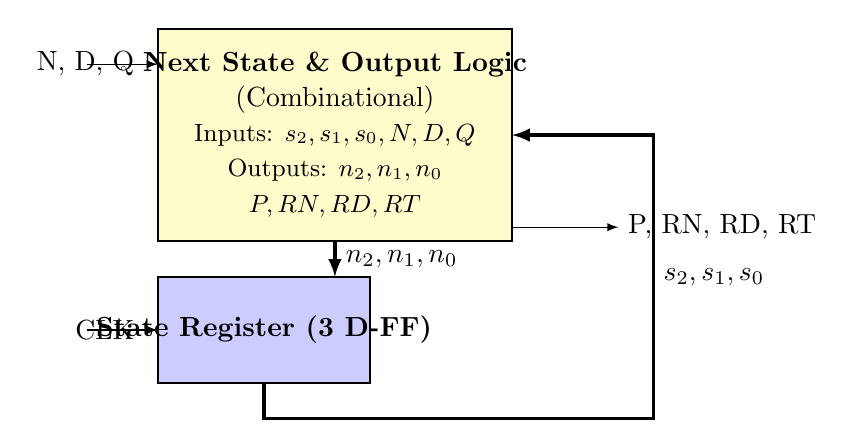
\begin{tikzpicture}[scale=0.9]
  % Combinational Logic Block
  \draw[thick, fill=yellow!20] (0,2) rectangle (5,5);
  \node at (2.5,4.5) {\textbf{Next State \& Output Logic}};
  \node at (2.5,4) {(Combinational)};
  \node[font=\small] at (2.5,3.5) {Inputs: $s_2, s_1, s_0, N, D, Q$};
  \node[font=\small] at (2.5,3) {Outputs: $n_2, n_1, n_0$};
  \node[font=\small] at (2.5,2.5) {$P, RN, RD, RT$};

  % State Register
  \draw[thick, fill=blue!20] (0,0) rectangle (3,1.5);
  \node at (1.5,0.75) {\textbf{State Register (3 D-FF)}};

  % Arrows
  \draw[-latex, very thick] (2.5,2) -- (2.5,1.5) node[midway, right] {$n_2, n_1, n_0$};
  \draw[-latex, very thick] (1.5,0) -- (1.5,-0.5) -- (7,-0.5) -- (7,3.5) -- (5,3.5);
  \node[right] at (7,1.5) {$s_2, s_1, s_0$};

  % Clock
  \draw[-latex] (-1,0.75) -- (0,0.75) node[left, xshift=-5] {CLK};

  % Inputs
  \draw[-latex] (-1,4.5) -- (0,4.5) node[left, xshift=-5] {N, D, Q};

  % Outputs
  \draw[-latex] (5,2.2) -- (6.5,2.2) node[right] {P, RN, RD, RT};
\end{tikzpicture}
\caption{FSM Implementation Block Diagram}
\end{figure}

\newpage
\section{Question 3: Output Sequence Controller FSM (10 marks)}

\subsection{Problem Statement}

Design FSM with:
\begin{itemize}
  \item \textbf{Input:} S
  \item \textbf{Outputs:} x, y, z
  \item \textbf{Sequence:} 000 $\rightarrow$ 001 $\rightarrow$ 010 $\rightarrow$ 100 $\rightarrow$ repeat
  \item \textbf{Initial state:} 000
\end{itemize}

The output should change only on rising clock edge.

\subsection{Part (a): Stop and Reset Behavior}

\textbf{Requirement:} When $S=1$, stop the sequence. When $S$ returns to 0, restart from 000.

\subsubsection{State Diagram}

\begin{figure}[H]
\centering
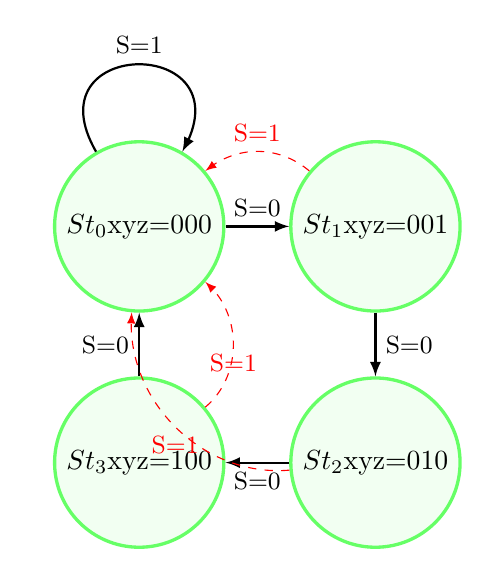
\begin{tikzpicture}[
  node distance=3cm,
  state/.style={circle, draw=green!60, fill=green!5, very thick, minimum size=1.8cm},
  >=latex
]

  % States
  \node[state] (St0) {$St_0$\\xyz=000};
  \node[state, right of=St0] (St1) {$St_1$\\xyz=001};
  \node[state, below of=St1] (St2) {$St_2$\\xyz=010};
  \node[state, left of=St2] (St3) {$St_3$\\xyz=100};

  % Normal transitions (S=0)
  \draw[->, thick] (St0) to node[above, font=\small] {S=0} (St1);
  \draw[->, thick] (St1) to node[right, font=\small] {S=0} (St2);
  \draw[->, thick] (St2) to node[below, font=\small] {S=0} (St3);
  \draw[->, thick] (St3) to node[left, font=\small] {S=0} (St0);

  % Reset transitions (S=1)
  \draw[->, dashed, red, bend right=40] (St1) to node[above, font=\small, red] {S=1} (St0);
  \draw[->, dashed, red, bend left=50] (St2) to node[below, font=\small, red] {S=1} (St0);
  \draw[->, dashed, red, bend right=50] (St3) to node[below, font=\small, red] {S=1} (St0);

  % Self loop for St0
  \draw[->, thick] (St0) to [out=120, in=60, looseness=4] node[above, font=\small] {S=1} (St0);

\end{tikzpicture}
\caption{FSM Part (a) - Stop and Reset State Diagram}
\end{figure}

\subsubsection{State Transition Table}

\begin{table}[H]
\centering
\caption{State Transition Table for Part (a)}
\begin{tabular}{c|c|c|c|ccc}
\toprule
\textbf{Current State} & \textbf{Code} & \textbf{S} & \textbf{Next State} & \textbf{x} & \textbf{y} & \textbf{z} \\
\midrule
$St_0$ & 00 & 0 & $St_1$ & 0 & 0 & 0 \\
$St_0$ & 00 & 1 & $St_0$ & 0 & 0 & 0 \\
$St_1$ & 01 & 0 & $St_2$ & 0 & 0 & 1 \\
$St_1$ & 01 & 1 & $St_0$ & 0 & 0 & 1 \\
$St_2$ & 10 & 0 & $St_3$ & 0 & 1 & 0 \\
$St_2$ & 10 & 1 & $St_0$ & 0 & 1 & 0 \\
$St_3$ & 11 & 0 & $St_0$ & 1 & 0 & 0 \\
$St_3$ & 11 & 1 & $St_0$ & 1 & 0 & 0 \\
\bottomrule
\end{tabular}
\end{table}

\subsubsection{Next State and Output Equations}

\textbf{State Encoding:} Using 2 bits $(s_1s_0)$
\begin{itemize}
  \item $St_0 = 00$
  \item $St_1 = 01$
  \item $St_2 = 10$
  \item $St_3 = 11$
\end{itemize}

\textbf{Next State Equations:}
\begin{align}
n_1 &= \overline{S} \cdot (s_1 \oplus s_0) \\
n_0 &= \overline{S} \cdot \overline{s_1} \cdot \overline{s_0}
\end{align}

\textbf{Output Equations:}
\begin{align}
x &= s_1 \cdot s_0 \quad \text{(output 1 only in $St_3$)} \\
y &= s_1 \cdot \overline{s_0} \quad \text{(output 1 only in $St_2$)} \\
z &= \overline{s_1} \cdot s_0 \quad \text{(output 1 only in $St_1$)}
\end{align}

\newpage
\subsection{Part (b): Postpone for 3 Cycles}

\textbf{Requirement:} When $S=1$, halt sequence for at least 3 cycles. When $S$ returns to 0 after 3 cycles, continue to next value.

\subsubsection{State Diagram}

\begin{figure}[H]
\centering
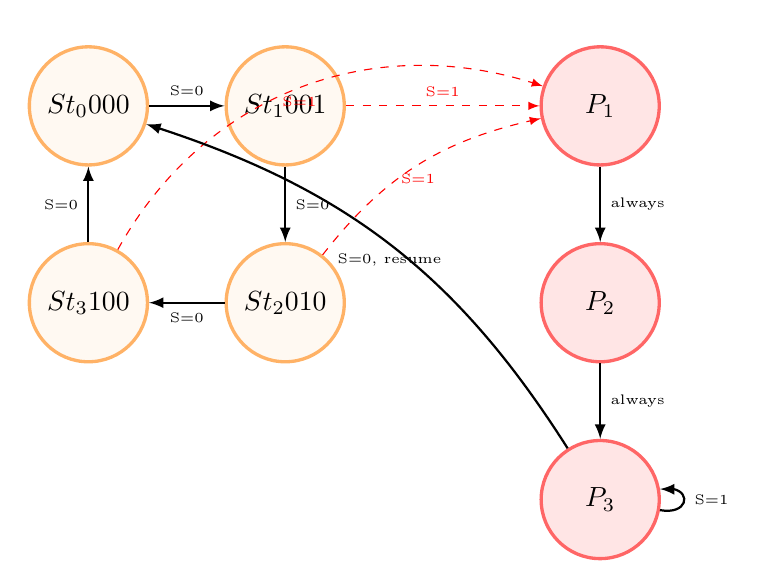
\begin{tikzpicture}[
  node distance=2.5cm,
  state/.style={circle, draw=orange!60, fill=orange!5, very thick, minimum size=1.5cm},
  pause/.style={circle, draw=red!60, fill=red!10, very thick, minimum size=1.5cm},
  >=latex
]

  % Normal States
  \node[state] (St0) {$St_0$\\000};
  \node[state, right of=St0] (St1) {$St_1$\\001};
  \node[state, below of=St1] (St2) {$St_2$\\010};
  \node[state, left of=St2] (St3) {$St_3$\\100};

  % Pause States
  \node[pause, right of=St1, xshift=1.5cm] (P1) {$P_1$};
  \node[pause, below of=P1] (P2) {$P_2$};
  \node[pause, below of=P2] (P3) {$P_3$};

  % Normal flow
  \draw[->, thick] (St0) to node[above, font=\tiny] {S=0} (St1);
  \draw[->, thick] (St1) to node[right, font=\tiny] {S=0} (St2);
  \draw[->, thick] (St2) to node[below, font=\tiny] {S=0} (St3);
  \draw[->, thick] (St3) to node[left, font=\tiny] {S=0} (St0);

  % Enter pause
  \draw[->, dashed, red] (St1) to node[above, font=\tiny] {S=1} (P1);
  \draw[->, dashed, red] (St2) to [bend left=20] node[below, font=\tiny] {S=1} (P1);
  \draw[->, dashed, red] (St3) to [bend left=40] node[below, font=\tiny] {S=1} (P1);

  % Pause progression
  \draw[->, thick] (P1) to node[right, font=\tiny] {always} (P2);
  \draw[->, thick] (P2) to node[right, font=\tiny] {always} (P3);

  % Resume
  \draw[->, thick, bend right=20] (P3) to node[below, font=\tiny] {S=0, resume} (St0);

  % Stay in pause
  \draw[->, thick] (P3) to [out=350, in=10, looseness=4] node[right, font=\tiny] {S=1} (P3);

\end{tikzpicture}
\caption{FSM Part (b) - 3-Cycle Postpone State Diagram}
\end{figure}

\subsection{Part (c): Postpone for 30 Cycles Using Counter}

\textbf{Requirement:} When $S=1$, halt for at least 30 cycles. After 30 cycles and $S=0$, continue to next value. Use MSI component to keep FSM simple.

\subsubsection{System Architecture}

\begin{figure}[H]
\centering
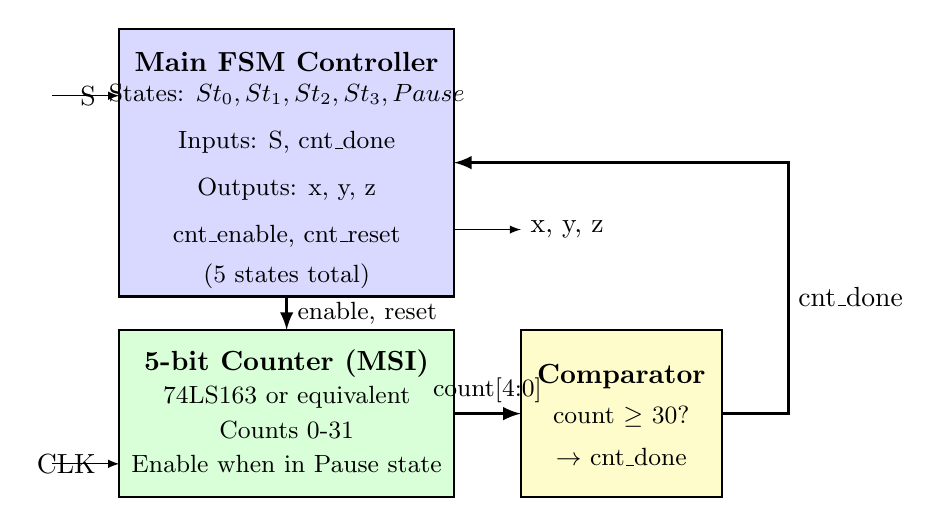
\begin{tikzpicture}[scale=0.85]
  % Main FSM
  \draw[thick, fill=blue!15] (0,3) rectangle (5,7);
  \node at (2.5,6.5) {\textbf{Main FSM Controller}};
  \node[font=\small] at (2.5,6) {States: $St_0, St_1, St_2, St_3, Pause$};
  \node[font=\small] at (2.5,5.3) {Inputs: S, cnt\_done};
  \node[font=\small] at (2.5,4.6) {Outputs: x, y, z};
  \node[font=\small] at (2.5,3.9) {cnt\_enable, cnt\_reset};
  \node[font=\small] at (2.5,3.3) {(5 states total)};

  % 5-bit Counter
  \draw[thick, fill=green!15] (0,0) rectangle (5,2.5);
  \node at (2.5,2) {\textbf{5-bit Counter (MSI)}};
  \node[font=\small] at (2.5,1.5) {74LS163 or equivalent};
  \node[font=\small] at (2.5,1) {Counts 0-31};
  \node[font=\small] at (2.5,0.5) {Enable when in Pause state};

  % Comparator
  \draw[thick, fill=yellow!20] (6,0) rectangle (9,2.5);
  \node at (7.5,1.8) {\textbf{Comparator}};
  \node[font=\small] at (7.5,1.2) {count $\geq$ 30?};
  \node[font=\small] at (7.5,0.6) {$\rightarrow$ cnt\_done};

  % Connections
  \draw[-latex, very thick] (2.5,3) -- (2.5,2.5) node[midway, right, font=\small] {enable, reset};
  \draw[-latex, very thick] (5,1.25) -- (6,1.25) node[midway, above, font=\small] {count[4:0]};
  \draw[-latex, very thick] (9,1.25) -- (10,1.25) -- (10,5) -- (5,5);
  \node[right] at (10,3) {cnt\_done};

  % Inputs
  \draw[-latex] (-1,6) -- (0,6) node[left, xshift=-5] {S};
  \draw[-latex] (-1,0.5) -- (0,0.5) node[left, xshift=-5] {CLK};

  % Outputs
  \draw[-latex] (5,4) -- (6,4) node[right] {x, y, z};

\end{tikzpicture}
\caption{FSM Part (c) - Complete System with Counter}
\end{figure}

\subsubsection{Operation Summary}

\textbf{Counter Logic:}
\begin{itemize}
  \item \textbf{Clock:} System clock (when cnt\_enable = 1)
  \item \textbf{Reset:} cnt\_reset signal from FSM
  \item \textbf{Output:} count[4:0] (5-bit value 0-31)
  \item \textbf{Compare:} cnt\_done = 1 when count $\geq$ 30
\end{itemize}

\textbf{Comparison Circuit:}
\[
\text{cnt\_done} = \text{count}[4] \cdot \text{count}[3] \cdot \text{count}[2] \cdot \text{count}[1]
\]

This is true when count = 30 (11110$_2$) or count = 31 (11111$_2$).

\textbf{Benefits of Using Counter:}
\begin{itemize}
  \item Main FSM remains simple (only 5 states instead of 33 states)
  \item Easy to modify pause duration (just change comparator value)
  \item Scalable to longer pause periods without adding states
  \item Uses standard MSI components (74LS163)
\end{itemize}

\newpage
\section{Summary and Conclusion}

\subsection{Key Concepts Learned}

\subsubsection{Question 1 - Decoder Implementation}
\begin{tcolorbox}[colback=green!5!white,colframe=green!75!black]
\textbf{Key Takeaways:}
\begin{itemize}
  \item Decoders generate minterms that can be combined to implement any Boolean function
  \item Hierarchical decoding: Using multiple small decoders (2×4) instead of one large decoder
  \item Enable input: Used to activate/deactivate decoder sections
  \item OR gate combination: Multiple decoder outputs ORed together for each function output
\end{itemize}
\end{tcolorbox}

\subsubsection{Question 2 - FSM for Sequential Control}
\begin{tcolorbox}[colback=blue!5!white,colframe=blue!75!black]
\textbf{Key Takeaways:}
\begin{itemize}
  \item FSM tracks accumulated state (vending machine requires tracking money accumulated)
  \item Moore Machine: Outputs depend only on current state
  \item State minimization: Only track necessary amount levels (0, 5, 10, 15, 20 cents)
  \item Change calculation: Logic to determine correct change based on overpayment
\end{itemize}
\end{tcolorbox}

\subsubsection{Question 3 - Advanced FSM Design}
\begin{tcolorbox}[colback=orange!5!white,colframe=orange!75!black]
\textbf{Key Takeaways:}
\begin{itemize}
  \item Output sequence generation: Using states to produce specific output patterns
  \item Input control: Modifying FSM behavior based on control input (S)
  \item Counter integration: Using MSI components to extend FSM capabilities
  \item Scalability: Part (c) shows how hardware design scales for larger requirements
\end{itemize}
\end{tcolorbox}

\subsection{Design Principles Applied}

\begin{enumerate}
  \item \textbf{Hierarchical Design:} Breaking complex circuits into manageable sub-blocks
  \item \textbf{State Minimization:} Using only necessary states to reduce complexity
  \item \textbf{MSI Integration:} Leveraging standard components (decoders, counters) for efficient designs
  \item \textbf{Verification:} Testing with multiple cases to ensure correctness
  \item \textbf{Documentation:} Clear diagrams, tables, and equations for understanding
\end{enumerate}

\subsection{Recommended Practice Problems}

\begin{enumerate}
  \item Design a traffic light controller FSM for a 4-way intersection
  \item Implement a sequence detector for pattern "1011" using FSM
  \item Create a digital lock with 4-digit code entry system
  \item Design an elevator controller FSM for a 3-floor building
  \item Implement a binary multiplier using decoders and adders
\end{enumerate}

\begin{tcolorbox}[colback=red!5!white,colframe=red!75!black,title=Final Note]
This solution provides comprehensive coverage of Digital System Design fundamentals including:
\begin{itemize}
  \item Combinational logic design using decoders
  \item Finite state machine design and implementation
  \item Integration of MSI components
  \item Professional circuit diagrams and documentation
\end{itemize}

\textbf{Your investment in understanding this material will benefit you throughout your engineering career!}
\end{tcolorbox}

\vfill
\begin{center}
\textbf{\Large END OF SOLUTION}\\
\vspace{0.5cm}
\textit{Digital System Design - Spring 2026 - CPE344}
\end{center}

\end{document}
